\documentclass[preprint,3p]{elsarticle}
%\documentclass[preprint]{aastex}
\usepackage{aas_macros}
\usepackage{amsmath,amssymb}
\usepackage{mathrsfs}
\usepackage{graphicx}
\usepackage{bm}
\usepackage{hyperref}

\newcommand{\mli}[1]{\mathit{#1}}
%\usepackage{epstopdf}


\begin{document}

\begin{frontmatter}

\title{Standard Candle Cosmology With Incomplete Spectroscopic Classification}
\author{A.~G. Kim\corref{cor1}}
\ead{agkim@lbl.gov}
\address{Physics Division, Lawrence Berkeley National Laboratory, 1 Cyclotron Road, Berkeley CA, USA 94720}

\begin{abstract}
\end{abstract}
\begin{keyword}
\end{keyword}
\end{frontmatter}

\section{Introduction}
A class of astronomical objects who share a common luminosity are called a standard
candle.  The relative fluxes (or magnitudes) for a set of these objects distributed in space
provide a measurement of their relative luminosity distances. These data, combined with
measurements of the standard candle redshifts, constitute a Hubble
diagram which is used to map the expansion history of the Universe.

Type~Ia supernovae (SNe~Ia) are an example of a standard candle (more precisely a standardizable
candle), whose redshift-magnitude relation provides an accurate expansion history
used to measure the Hubble Constant
\citep{2001ApJ...553...47F} and detect the accelerated expansion of the Universe
\citep{1998AJ....116.1009R, 1999ApJ...517..565P}.  SN~Ia measurements continue
to improve 
\citep{2014A&A...568A..22B} and play a critical role in probing the physics
responsible for the acceleration \citep{2013PhR...530...87W}.
Looking at the present and toward the future, SN~Ia cosmology is
a component of the Dark Energy Survey\footnote{\url{http://www.darkenergysurvey.org}} (DES),
and a science driver in the design of the
Large Synoptic Survey Telescope\footnote{\url{http://www.lsst.org}} (LSST)
and the Wide-Field InfrarRed Survey Telescope
\citep{2015arXiv150303757S}.

The information necessary to construct a Hubble diagram consists of, per object,
its classification as a
member of the standard candle class, its redshift, and its flux.  For SNe~Ia, the flux at
peak brightness is typically determined from multi-band light curves obtained from repeated
photometric observations. Traditionally, spectroscopic data is used to classify the transient
as SN~Ia through the lack of hydrogen and the presence of SiII in its spectrum,
and determine its redshift either directly through the transient spectrum or that of its host
galaxy. While the classification and redshift could be determined from the multi-band
light curves and colors of the host galaxy, the accuracy is insufficient for precision
cosmology \citep{2011ApJ...738..162S}.  Consequently spectroscopic follow-up
has played a critical role in cosmological supernova surveys.

While the large focal planes of the Dark Energy Camera (3 square degrees)
and the LSST (9.6 square degrees) open the
possibility for the photometric discovery and observation of thousands to millions
of SNe~Ia out to $z\sim1$, a corresponding multiplex advantage has not been
achieved for the 10-m
class telescopes used for the spectroscopic classification of faint discoveries:
it is unfeasible to obtain a spectrum for all SN~Ia candidates with well-measured
photometry.

Photometric supernova analysis has been proposed to  take advantage of the statistical weight imported by large numbers of supernova light curves, despite the lack of spectroscopy.
An example of such a program would proceed as follows: A rolling wide-field imaging
survey generates light curves for all transients in the survey area.  In near real-time,
a subset 
of transients from those images are selected for triggered spectroscopic observations
to obtain classifications and redshifts.  At the end of the survey, the
analysis sample is the subset of likely SN~Ia
candidates based on photometric data;  the analysis sample and its subset
with triggered spectroscopy are constructed so as to be drawn from the same parent distribution.
Spectroscopic redshifts are obtained for likely host galaxies.  The Hubble diagram of the
analysis sample is analyzed with the understanding that it may contain multiple populations.

The Sloan Digital Sky Survey-II Supernova Survey is an example of a program
that produced significant numbers of transients
with light curves but without spectroscopic typing \citep{2014arXiv1401.3317S}:
photometric SN analysis has been developed applied to these data \citep{2012ApJ...752...79H,
2013ApJ...763...88C}.   Such analyses are anticipated in the projected
supernova programs of 
DES \citep{2012ApJ...753..152B} and LSST \citep{2012arXiv1211.0310L}.

Current models used for supernova cosmology analysis account for unobserved quantities.
SNe~Ia are not standard but are ``standardizable'' candles, implying that the class may be composed of distinct subpopulations each with its own redshift-dependent rates, magnitude distributions, and secondary
observable (e.g.\ light-curve shape, color) distributions.  Bayesian hierarchical modeling is 
used to account for this extra layer of complexity  to determine characteristics of the SN~Ia population simultaneously
with the cosmology \citep{2011MNRAS.418.2308M,
2015arXiv150701602R}.  Consideration of missing classification is addressed
by
BEAMS \citep{2007PhRvD..75j3508K}, which  includes a non-Ia population in sample, whose luminosity distribution
is inferred along with the cosmology:
BEAMS was used in the analysis of SDSS-II SN data \citep{2012ApJ...752...79H}.

This article addresses the affect of missing spectroscopic typing in
a transient standard candle analysis, with the eventual goal of quantifying
requirements for the spectroscopic subsample in a broader photometric analysis.
The lack of spectroscopy leads to ambiguity in both the transient class and
in the host galaxy due to projected galaxies that appear close to the transient or
the relative low-surface brightness of the host.  The subsample with
spectroscopic typing informs the interpretation of objects lacking spectroscopy.
Differences between observed and
intrinsic distributions in a flux-limited sample can have important effects on the Hubble
diagram  (e.g.\ Malmquist bias) so are accounted for explicitly.

\section{DES SN Survey Model}
\label{snIamodel:sec}
\subsection{Model}
\label{model:sec}
This Section presents a candidate model
for supernova surveys that has the fidelity needed for the photometric
supernova analysis of the Dark Energy Survey and the Large Synoptic Survey Telescope.
This model captures the current treatment in current analyses and is expanded to include
photometry-only transients.  This may not be the ultimate model used, indeed many models
need to be considered for model testing.

The Probabilistic Graphical Model is shown in Figure~\ref{pgm:fig}. The underlying behavior of the universe is described by the following elements:
\begin{description}
\item [Cosmology] Luminosity distance for the cosmological model being considered,
e.g.\ a $wCDM$ universe parameterized by $\Omega_M$, $\Omega_w$, $w_0$, $w_a$.
\item[SNe~Ia, Non-Ia Populations] Time-dependent luminosity for all transient populations
that may enter
the analysis.  The SALT2 model is a candidate for SNe~Ia, with parameters $\alpha$, $\beta$.  The PSNID treatment of non-Ia's can be made into a model for the other
transients or Natahsa Karpenka is working on a model of non-Type~II core collapse SNe.
\item [Relative Rates] Relative rates of all the transients populations and
subpopulations (e.g. SALT2 $x_1$, $c$) under consideration.  The
model could of been extended to measure absolute rates, but that is unnecessary if
the cosmological parameters are the goal.
\end{description}
Each transient is described by the following elements:
\begin{description}
\item[Host Galaxy] The host galaxy, or more generally for the case of hostless supernovae,
the environment from which the transient arises.  The host is described by its redshift
and other parameters that may be of interest such as mass,
specific star formation rate, metallicity.
\item[Type Subtype] Specification of the the transient: the population to which it belongs
and its internal parameters.  For example, an object could be SN~Ia with specific
values for its SALT2 parameters $c$, $x_1$, $t_0$ and its random dispersion
realization (both absolute magnitude and from the error snake). 
This is dependent on the relative rates and
its host galaxy including its redshift.
\item[Distance] Distance modulus or equivalently the luminosity distance of the host galaxy,
which in our model corresponds to the cosmological redshift of the transient.  The value
is fixed based on the cosmology and redshift.
\end{description}
The individual photometric measurements of a transient are described by the following
elements:
\begin{description}
\item[Luminosity]  Luminosity as a function of wavelength
corresponding to the date of observation.   This depends on the population, type,
and subtype.  Given that searching for correlations between  host properties and Hubble
residuals is a good probe of systematics,
a direction connection between host galaxy and luminosity is made.
\item[Flux] Flux of the transient incident to earth at the date of observation.  It is 
fixed based on the luminosity, redshift, and distance.
\end{description}
The observatory is described by the following element:
\begin{description}
\item[Throughput] The transmission function experienced by the transient during
the observation.  It depends on band, position on the focal plane, and date of observation.
\end{description}
The data (subscripted by ``o'' for observation)  are:
\begin{description}
\item[$\text{Photometry}_o$] Photometric flux measurement of the transient.
The expected measurement
is the incident flux integrated over the throughput.
\item[$\text{Type Subtype}_o$] Spectroscopic
measurements of the intrinsic transient type.  It is dependent on the underlying
type.
\item[$\text{Redshift}_o$] Measurement of the host redshift.  The redshift can be
spectroscopic or photometric.  It is dependent on the host redshift, and
redshifts of any other galaxies that may be confused as the host (not shown explicitly
in the PGM).
\item[$\text{Host Properties}_o$] Measurement of the host properties such
as mass, sSFR, metallicity. It is dependent on the host galaxy, and
any other galaxies that may be confused as the host.
\end{description}


\begin{figure}[htbp] %  figure placement: here, top, bottom, or page
   \centering
   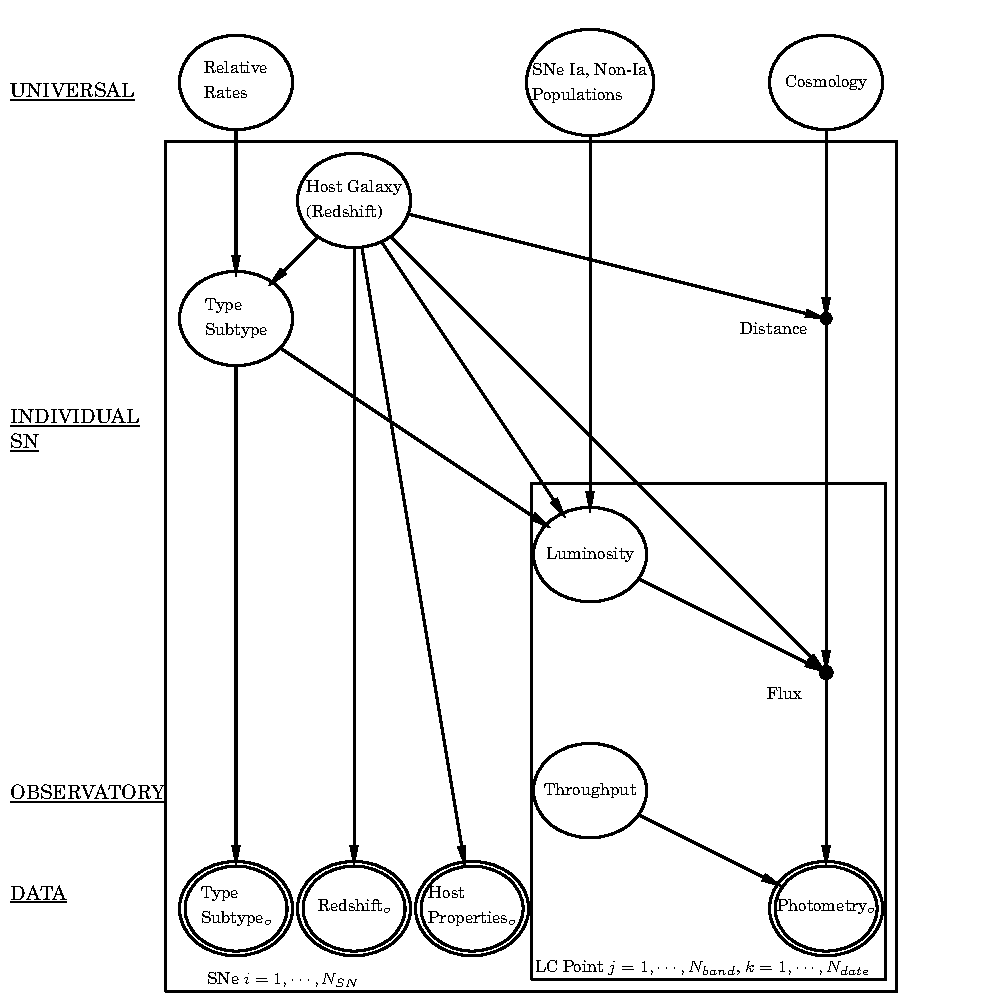
\includegraphics[width=6.5in]{/Users/akim/project/abc/results/hdpgm.pdf} 
   \caption{Probabilistic Graphical Model for the SN~Ia analysis.  
   The description of the elements and dependencies of the model are given in
   \S\ref{model:sec}.
   \label{pgm:fig}}
\end{figure}

This hierarchical model has several features worth noting.  Transients with and without
spectroscopic classification are treated together: those with classification help constrain
the properties of the underlying population to inform the treatment of those without.
Photometric classification is treated internally, through the
latent Type.  The system throughput is treated as a probabilistic variable
allowing for self-calibration; this could be omitted from the model with calibration
and its uncertainties applied
to the Photometry measurements.  Host-galaxy misclassification enters as measurement
uncertainties.  Malmquist bias and other selection effects do not appear explicitly, but are accounted
for in the likelihoods.  The model could be extended to include summary statistics,
for example the results of an external supernova classifier; the use
of summary statistics would affect the manner in which the model is evaluated
due to our inability to write their likelihoods.

\subsection{Sample Selection}
The transients that enter the analysis satisfy some selection criteria.  Trivially, they
have to be discovered in the first place and often more stringent photometric signal-to-noise
requirements are applied.  Additionally, transients that have
successful spectroscopy may be drawn from an underlying population that differs from the
underlying or photometrically-selected samples.

Sample selection criteria for DES have not yet been finalized
(Argonne Eve for photometry, OzDES/Ryan for spectroscopy are candidates to do this);
presented here is a sketch of the likelihood calculation for a reasonable
photometric selection criterion:
for each transient $\nu$, the criterion is to have $\ge N$ photometric points
above a signal-to-noise threshold given $M_\nu$ available measurements.
Each photometric point is associated with a flux threshold that it either passes
or fails.  Given a total $M=\sum_\nu M_\nu$ data points, there are
$2^M$ possible configurations
of the individual points passing or failing theshold, of which only
$\prod_\nu \sum_{k=N}^{M_{\nu}} \binom{M_{\nu}}{k}$  configurations lead to
the inclusion of the transients in the sample.

The likelihood for the analysis
sample is the conditional distribution obtained by applying the selection criteria
on the domain of the likelihood given no selection criteria.  This latter likelihood
can be written
as the sum of the contributions from all possible threshold-passing configurations
\begin{equation}
p(data|model) = \sum_{k=1}^{2^M} p(data, \hat{b}_k| model),
\label{likelihood_u:eqn}
\end{equation}
where $\hat{b}$ is the set containing all possible configurations.
Let $b$ be the subset of $\hat{b}$ 
that satisfies sample selection. Then the selection criteria is $\mathcal{S} = \hat{b}_k
\in b$.
The likelihood of the analysis sample is proportional to Eqn.~\ref{likelihood_u:eqn}
with failing configurations removed
\begin{equation}
\mathcal{L}(data|\mathcal{S}, model) =
\sum_{k=1}^{2^M} p(data, \hat{b}_k| \hat{b}_k
\in b, model) \propto \sum_{k=1}^{\prod_\nu \sum_{k=N}^{M_{\nu}} \binom{M_{\nu}}{k}} p(data, b_k| model),
\end{equation}


The probability for the data to be in a specific configuration $b_k$ of
being below or above flux threshold is expressed
as
\begin{equation}
p(data, b_k| model)  = \epsilon(Photometry_o, b_k)p(data| model)\\
\end{equation}
where
\begin{equation}
\epsilon(Photometry_o; b_{k})= \prod_{\nu i}\mathcal{H}\left((-1)^{b_{k\nu i}+1}(Photometry_{o,k\nu i}-Threshold_{\nu i})\right),
\label{eff:eqn}
\end{equation}
where $\mathcal{H}$ is the Heaviside step function; when $b_{k\nu i}=1/0$ the step in the efficiency
is up/down.  The indices correspond to configuration $k$,
transient $\nu$, and photometric point $i$.

Assembling this together, the likelihood is
\begin{equation}
\mathcal{L}(data|\mathcal{S}, model) = \frac{\sum_{k=1}^{\prod_\nu \sum_{k=N}^{M_{\nu}} \binom{M_{\nu}}{k}} \epsilon(Photometry_o, b_k)p(data| model)}{\int ddata\,
\sum_{k=1}^{\prod_\nu \sum_{k=N}^{M_{\nu}} \binom{M_{\nu}}{k}} \epsilon(Photometry_o, b_k)p(data| model)
}
\end{equation}
where the normalizing factor is included explicitly as it has 
parameter dependence and must not be neglected in calculations.

Consider the traditional case of Malmquist bias of a single object,
where a single measurement has
to be above flux threshold.  For the underlying distribution with no flux threshold there
are $2^1=2$ possible configurations, the flux is either above or below threshold.  For
the sample distribution, there is $\binom{1}{1}=1$ possible configuration: the flux
is above threshold.   The likelihood for the measured flux is proportional to the original
distribution truncated so that fluxes below threshold are assigned zero probability.

For the case of a single object with two measurements of which only one is needed to
pass threshold,
there are $2^2=4$ possible configurations of which $\sum_{k=1}^{2} \binom{2}{k}=3$
allow sample selection, the exception being when both measurements fall below threshold.
The likelihood for each flux is composed from
the sum of three truncated distributions of which one accepts faint fluxes,
resulting in likelihoods that are not zero below detection threshold.

\subsection{Underlying Likelihood}
The likelihood of the analysis sample is calculated from the underlying pdf of data.  Based on Figure~\ref{pgm:fig},
\begin{align}
p(data|model) &=\int dType\, dLuminosity\, p(Photometry_o |  Luminosity, Cosmology,Host,Throughput)  \nonumber\\
& p(Luminosity| Type
, Host, Population) p(Type | Rates, Host)  \nonumber\\
& \times \int dType\, p(Type_0|Type) p(Type|Rates, Host) \nonumber \\
& \times p(Redshift_o, Host_o| Host),
\label{like:eqn}
\end{align}
where $data=\{Photometry_o, Type_o, Redshift_o, Host_o\}$,
$model=\{Cosmology, Populations, Rates\}$, and the independence
of photometric and spectroscopic typing measurements is anticipated.

For specificity candidate models for the pdf's that appear in Eqn.~\ref{like:eqn}
are now presented.
\begin{itemize}
\item The type is drawn from the host-dependent relative rate between SNe~Ia and non-Ia's 
\begin{equation}
Type | Rates, Host \sim {\rm Bernoulli}(\pi(z;r)),
\end{equation}
where $\pi$ is a model for the relative rate of SNe~Ia parameterized by $r$ as a
function of galaxy redshift $z$.  {\bf A reasonable choice for $\pi$ needs to be
selected.}

Type~Ia supernovae have values of SALT2 parameters
$x_1$ and $c$ drawn from Normal distributions
with parameters for the variance
\begin{equation}
x_1, c \sim \mathcal{N}(0, (\sigma_{x_1}, \sigma_c)).
\end{equation}

Models for non-Ia supernovae need to be selected. 

Note that the rates may not have been important in spectroscopic analyses, but are important here to help infer the types/subtypes of transients without
a spectrum.
\item For the underlying SED of transients for SNe~Ia the SALT2 model
is an option, although new models are expected to appear shortly.  Absolute magnitudes
that depend on host-galaxy properties also need to be considered. 
In the SALT2 context,
\begin{equation}
Luminosity(Type
, Host, Population)= L_{SALT2}\left(\frac{t-t_0}{1+z}; \alpha, \beta, x_1, c\right) \exp{\left(\delta_G\mathcal{H}(g)\right)},
\end{equation}
where the first  term is the SALT2 light-curve and absolute magnitude
model with error snake.  Possible host-galaxy effects like the ``mass step'' are
accounted in $\mathcal{H}(g)$ where $g$ is the corresponding host parameter
and $\delta_G$ is the size of the offset.  The host redshift is $z$.
Note that for this model the parameter is fixed, though
generally this may not be the case.

{\bf The non-Ia model needs to be identified.}
\item The theoretical distance modulus is
\begin{equation}
\mu(Host, Cosmology) = \mu_{wCDM}(z; \Omega_M, w)
\end{equation}
is the predicted distance modulus of a flat dark energy cosmology
with parameters $\Omega_M$ and $w$, and host redshift $z$.

The flux incident on Earth is the redshifted and time-dilated SED scaled
by the distance modulus
\begin{equation}
f(Luminosity, Host, \mu) = 10^{-\mu/2.5} Luminosity(\lambda/(1+z)).
\end{equation}

The expected photometric signal in counts depends on the flux and throughput of the
optical chain.  A simple model encapsulates flux calibration through a zeropoint $Z$
and $T_0$  a fiducial transmission function for the appropriate filter.
More
sophisticated descriptions of calibration can vary the shape, not only the normalization, of the
transmission.  For the simple model,
\begin{equation}
counts(Throughput, f) = 10^{Z/2.5} \int  f(\lambda) T_0(\lambda)d\lambda.
\end{equation}

Practically the photometric extraction is handled by independent software, which calculates
the integrated counts with uncertainties $C_P$
by modeling and separating out polluting background light from the transient
signal
\begin{equation}
Photometry_o |  Luminosity, Cosmology,Host,Throughput \sim \mathcal{N}(counts,C_P).
\end{equation}
Dillon is providing this $Photometry_o$ and $C_P$.

An alternative model would be to remove Throughput
and include calibration uncertainties in $C_P$.  This would be a huge covariance
matrix!
\item Spectroscopic measurements are assumed
to provide prefect determinations of transient type
\begin{equation}
Type_o(Type)  = Type.
\end{equation}
\item There are measurements of the host galaxy properties.
For transients that have spectroscopic
confirmation, an unambiguous host determination is assumed such that
\begin{align}
Redshift_o(Host) & = z\\
Host~properties_o  | Host & \sim \mathcal{N}(p, C),
\end{align}
where $p$ are the Host properties being measured
and
$C$ their measurement uncertainty.

For the photometric sample, there is uncertainty in the identity of the host galaxy.
Suppose host-galaxy identification gives
a set of potential hosts $\hat{G}$ each with probability $\pi$ of being the correct host,
what Ravi is doing.
Then for the photometric sample
\begin{equation}
p(Redshift_o, Host~properties_o   | Host) = \sum_i \pi_i \delta(Redshift_o- z_i)\mathcal{N}(Host~properties_o-p_i, C)).
\end{equation}
Recall that DES plans to get spectroscopic redshifts with negligible measurement uncertainties on all
possible hosts.
\end{itemize}


This accounts for all the terms needed to assemble to pdf of the underlying distribution,
from which the likelihood of the analysis sample is assembled.


\section{Tasks}
Here are a list of initial tasks and ingredients needed to proceed.
\subsection{Photometric Selection}
Here are desired properties of the set (or sets) of objects obtained from photometric selection.
\begin{itemize}
\item Sufficient data-quality to have a chance at photometric classification.
SNe~Ia do look different from other transients: the principal source of type  ambiguity
comes from poor signal-to-noise and poor temporal/wavelength sampling.
Having enough points with sufficient signal-to-noise over three adjacent bands over a 
sufficiently large time window.
\item A large set of likely SNe~Ia.
\item All objects with photometry-only must have spectroscopically-typed analogs, preferably though not necessarily at the same redshift.  SNe~Ia subpopulations whose characteristics
are unconstrained are not useful for cosmology.
\item Obvious non-Ia's from populations that could be misconstrued as SN~Ia.  For example,
a non-Ia at low redshift could be
mistaken to be SN~Ia at high redshift due to degraded signal.  
\item Exclusion of objects that are not part of populations that could be misconstrued as SN~Ia.
They would pollute inference of the non-Ia population.
\end{itemize}

\subsection{Detection Criteria (Malmquist Bias)}
The photometric selection criteria are expected to be significantly more rigorous that
the detection criteria.  Nevertheless, the detection efficiencies need to be characterized.
Fakes already provide a good measure of this.  To first order, the efficiency depends
on $S/N$, but a secondary dependence on the structure of background galaxies.
The detection efficiency is more complicated than the step function
shown in Eqn.~\ref{eff:eqn}.

Deliverable is the detection efficiency to take the place of Eqn.~\ref{eff:eqn}.

\subsection{Per-Exposure Thresholds}
To understand the effect of sample-selection criteria and detection efficiency
on a specific object, the
properties of each photometric point is needed.  Although the photometric criteria
have not been formalized, a $S/N$ threshold is a possible statistic to be used.
As such, a clean deliverable would be:
\begin{itemize}
\item Determination of flux thresholds for each photometric point of each candidate
given
a $S/N$
\begin{equation}
threshold(point, S/N).
\end{equation}
If we work in the sky-noise dominated regime, I believe this information is already
calculated by DM.
\end{itemize}

\subsection{Spectroscopic Selection}
Identification of selection criteria for spectroscopic success, as a function
of data.

\subsection{Relative Rates}
\label{rates:sec}
A rates model for transient types and subtypes
\begin{equation}
\pi(z;r).
\end{equation}
\subsection{SALT2}
Decision on how to model the distribution of $x_1$ and $c$.  For a first try a
single normal distribution seems sufficient but do we want to be more ambitious?
\subsection{Non-Ia Transient Model}
Needed is a model(s) for non-transients that could be mistaken as SN~Ia:
both a description of the time-evolving SED and the relative rates
with respect to Type~Ia's (see \S\ref{rates:sec}).

The SED model is of the time evolving luminosity (or more precisely $\mathcal{M}$)
for the range of possible non-Ia's.  It describes not only colors and light curve shapes,
but also absolute magnitude.  Its parameters can be constrained part of the
global analysis, indeed the pdf of the absolute magnitude is candidate.

As much of its usage is in classification, PSNID is a place to start.
Natasha Karpenka has been compiling a descriptions of non-Ia-Type~I's.  Can these
be packaged into the following deliverable?

The deliverable is a parameterized SED model that can be accessed through
an interface such as $L(t,\lambda; \text{Non-Ia parameters})$. 

\subsection{Host-Galaxy Parameter Determination}
Although a different group within DES is charged with deriving properties
of galaxies (including our hosts), results do not seem to be forthcoming.
Mat has said that there is a group within the SNWG interested in
taking over this task.  Chris has discussed getting deep
co-adds of galaxies uncontaminated by supernova light.
Can we confirm who is part of this effort, if there is forward momentum,
and get a single name that used as the point of contact?

The deliverable are galaxy properties and a covariance matrix of their uncertainties,
which are treated in the analysis as data.

\subsection{NIR Data}
VISTA NIR data have important probative value that can enhance about all aspects
of our analysis even if available for a subset of objects.
We should decide our intents on the timing of the use of this data.
For example, on whether we plan on a DES-only paper and DES+NIR, and if
we want to focus efforts on the former in the short term.

\subsection{Photometric Data}

Deliverable:
transient counts and associated covariance matrix.  For flexibility, the counts and the
flux calibration are delivered separately.

\subsection{Calibration model and uncertainties}
For the first analysis, it is presumably sufficient to describe calibration uncertainties
as global zeropoints.  In the long term, it would be great to have a transmission
function for every photometric point.

It has to be decided whether calibration should be included
as part of the photometric uncertainties, or as model parameters.
The former requires the inversion of a full covariance matrix for all photometric
points.  The latter may have a per-SN solution through importance sampling.

Deliverable of $p(Z)$.

\subsection{Others}

\begin{itemize}
\item Data! Spectroscopic Type and uncertainties, Spectroscopic redshifts and
uncertainties, galaxy properties and uncertainties, host-galaxy associations
and uncertainties, photometry and uncertainties.
\item Determine the mechanics of doing the analysis.  A Bayesian MCMC could produce posteriors, which sampler that best suits our needs? Is a frequentist
analysis technically unfeasible? If redshifts were free to wander I would think so, but maybe
it is possible in this model.
\end{itemize}

%\section{Misc}
%The simulation of data from the model presented in
%and their analysis is implemented in Python and are available
%on GitHub\footnote{{git@github.com:AlexGKim/abc.git}}.
%
%
%\section{Standard Candle}
%\label{toy:sec}
%To introduce basic model elements, this Section considers a
%simplified view of SNe~Ia
%as transients that are bolometric standard candles with an intrinsic random
%dispersion
%at peak brightness, and assumes data with negligible measurement uncertainties.
%For convenience,
%the transients
%in this Section are  referred to as SNe~Ia.
%The added complexity of correlations between absolute magnitude
%and multi-band light curves, and measurement uncertainties
%are discussed in
%\S\ref{snIamodel:sec}. 
%
%\subsection{Base Model}
%\label{model:sec}
%This Section presents a model that is used both for generating simulated data, and for analysis.
%The data used to construct a Hubble diagram and the fundamental parameters of the
%model used to describe those data are succinctly summarized in the notation
%for the likelihood 
%\begin{equation}
%p(f, {{T}}_S,{{z}}_S, G|  \Omega_M, w, \theta_r,\alpha_{Ia},\sigma_{Ia}, \alpha_{\mathit{!Ia}},\sigma_{\mathit{!Ia}}),
%\label{likelihood:eqn}
%\end{equation}
%whose relations are sketched in the probabilistic graphical model in Figure~\ref{toypgm:fig}.
%The measurements are
%\begin{itemize}
%\item $f$: the flux at peak brightness, taken 
%to be bolometric to facilitate the treatment of
%standard candles at different redshift;
%\item ${{T}}_S$, ${{z}}_S$: the spectroscopic type and redshift available for a subset of transients;
%\item $\theta_{G1}$, $\theta_{G2}$: the spectroscopic redshifts of the galaxies identified
%as host and neighbor from imaging.
%\end{itemize}
%The model parameters are
%\begin{itemize}
%\item $\Omega_M$, $w$: the mass density and dark-energy equation of state parameters of a flat,
%constant-$w$ dark-energy cosmology;
%\item $\theta_{r1}$, $\theta_{r2}$:  the parameters
%that describe the redshift-dependent relative fraction of SNe~Ia and non-Ia's;
%\item $\alpha_{Ia}$, $\sigma_{Ia}$, $\alpha_{\mathit{!Ia}}$, $\sigma_{\mathit{!Ia}}$:
%the luminosity (times $4\pi$) and intrinsic dispersion for SNe~Ia and non-Ia at peak brightness.
%\end{itemize}
%Not listed explicitly in Eqn.~\ref{likelihood:eqn} but shown in Figure~\ref{toypgm:fig} are latent model parameters for each transient:
%\begin{itemize}
%\item $z$: the cosmological redshifts of the host and neighboring galaxies;
%\item $T$: the class of the objects, SN~Ia or non-Ia;
%\item $L$: the luminosity of the transient.
%\end{itemize}
%There is a  fixed parameter
%\begin{itemize}
%\item $\mu$: the distance modulus given the cosmological parameters and the redshift.
%\end{itemize}
%
%\begin{figure}[htbp] %  figure placement: here, top, bottom, or page
%   \centering
%   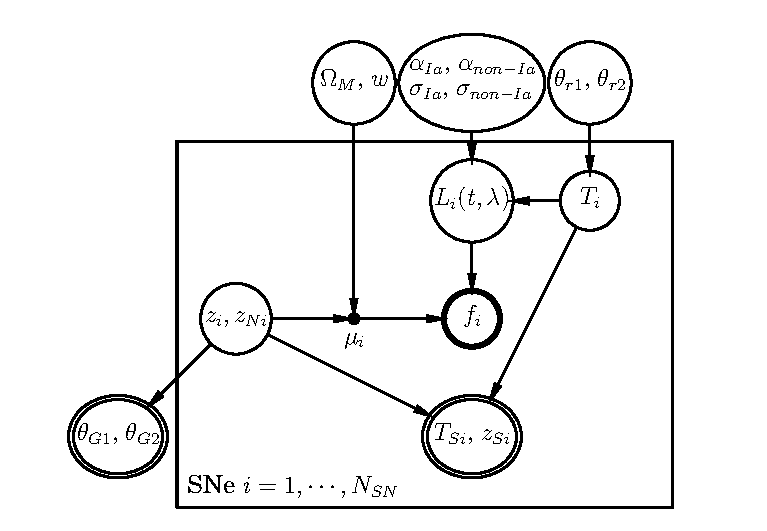
\includegraphics[width=4.5in]{/Users/akim/project/abc/results/toy_pgm.pdf} 
%   \caption{Probabilistic Graphical Model for the standard candle analysis. The
%   parameters include the cosmological parameters $\Omega_M$ and $w$,
%   the luminosities $\alpha$ and intrinsic dispersions $\sigma$ of SNe~Ia and non-Ia's,
%   and the relative fraction parameters $\theta_{r1}$ and $\theta_{r2}$.  Latent parameters
%   include 
%   for each transient the type $T$ and redshifts of the host and neighboring galaxies $z$ and $z_N$.  The  distance modulus $\mu$ and
%   luminosity $L$ are fixed by the other parameters.  The observables include the measured
%   flux $f$, spectroscopic type and redshift $T_S$ and $z_S$, and
%   the inferred host and neighbor redshifts $\theta_{G1}$ and $\theta_{G2}$.
%   The host and neighbor galaxies of all transients are inferred based a common galaxy catalog, 
%   and so strictly are not independent from supernova to supernova.
%   \label{toypgm:fig}}
%\end{figure}
%
%
%The transients being analyzed have passed some detection threshold
%and thus are drawn from
%distributions that have different shapes than the underlying population of both discovered and
%non-discovered objects. A  threshold flux of $f_0$ is adopted for the detection criterion.
%Otherwise, no other sample-selection criteria are assumed.
%
%\subsubsection{Likelihood for the {\it obs} set data}
%\label{obs:sec}
%The likelihood of data from the {\it obs} set, which has
%spectroscopic observations $T_S$ and redshift
%$z_S$, is described as follow.  The likelihood is
%\begin{align}
%p(f, {{T}}_S,{{z}}_S|  \Omega_M, w, \theta_r,\alpha_{Ia},\sigma_{Ia}, \alpha_{\mathit{!Ia}},\sigma_{\mathit{!Ia}}, z)  &=\sum_T
%p(f, {{T}}_S,{{z}}_S, T| \ldots)\\
%&= \sum_T 
%p(f, {{T}}_S,{{z}}_S| T,\dots) p(T | \ldots).
%\end{align}
%
%Direct associations between model and spectroscopic redshift and type are made
%\begin{align}
%p(z_S|z) &= \delta(z_S-z)\\
%p(T_S|T) &= \delta(T_S-T),
%\label{specz:eqn}
%\end{align}
%so that
%\begin{align}
%p(f, {{T}}_S,{{z}}_S|  \ldots) &= 
%p(f| T=T_S, z=z_s,\dots) p(T_S|z=z_s, \ldots).
%\label{obs:eqn}
%\end{align}
%
%
%The first term describes the expected counts. Given the redshift
%and transient type, the brightness of the underlying population
%is modeled as being drawn from a standard candle
%with mean luminosity $4\pi\alpha_X$ and a normal distribution in magnitude
%space with intrinsic dispersion  $\sigma_X$:
%\begin{equation}
%f| T=T_S, z=z_S, \Omega_M, w, \theta_r, \alpha_{Ia},\sigma_{Ia}, \alpha_{\mathit{!Ia}},\sigma_{\mathit{!Ia}} \sim \mathcal{N}_{\ln}\left(\ln{\left(\frac{\alpha_{T_S}}{d_L^2(z_S;\Omega_M, w)}\right)}, \frac{\ln{10}}{2.5}\sigma_{T_S}\right),
%\label{flux:eqn}
%\end{equation}
%where $\mathcal{N}_{\ln}$ is the log-normal distribution and $d_L$ is the luminosity distance.
%Measurement uncertainty is taken to be negligible.
%In a flux-limited survey, the pdf's for the data are truncated versions of the underlying
%pdf's.
%\begin{itemize}
%\item For SNe~Ia  $T_S=1$:
%\begin{equation}
%f | T=1, z=z_S, \Omega_M, w, \alpha_{Ia},\sigma_{Ia} \sim
%\frac{\mathcal{N}_{\ln}\left(\ln{\left(\frac{\alpha_{Ia}}{d_L^2(z_S;\Omega_M, w)}\right)}, \frac{\ln{10}}{2.5}\sigma_{Ia}\right)}{P_{Ia}(f > f_0)}.
%\label{adusnIa:eqn}
%\end{equation}
%\item For non-Ia's in set $T_S=0$:
%\begin{equation}
%f | T=0, z=z_S, \Omega_M, w, \alpha_{\mathit{!Ia}},\sigma_{\mathit{!Ia}}\sim 
%\frac{\mathcal{N}_{\ln}\left(\ln{\left(\frac{\alpha_{\mathit{!Ia}}}{d_L^2(z_S;\Omega_M, w)}\right)}, \frac{\ln{10}}{2.5}\sigma_{\mathit{!Ia}}\right)}{P_{!Ia}(f > f_0)},
%\label{adunonIa:eqn}
%\end{equation}
%\end{itemize}
%where the normalization factor is the complementary cumulative distribution function
%for the corresponding log-normal distribution that accounts for the truncated
%distribution of the detected sample.
%It is understood implicitly that as all objects must pass the detection threshold,
%the case of $f<f_0$ is never confronted in the analysis.
%
%The second term gives the type probability. In our model,
%the underlying relative rates between SNe~Ia and non-Ia are linear in redshift,
% parameterized by the
%its values at $z=0$ and $1.1 \times z_{max}$, 
%\begin{equation}
%\hat{\theta}_r=\theta_{r0}+z\left(\frac{\theta_{r1}-\theta_{r0}}{1.1 \times z_{max}}\right).
%\label{rate:eqn}
%\end{equation}
%The relative rate for SN~Ia discovery for the discovered (truncated) distribution is
%\begin{equation}
%\theta_r=\frac{\hat{\theta}_rP_{Ia}(f > f_0)}{\hat{\theta}_{r}P_{Ia}(f > f_0) + (1-\hat{\theta}_{r})P_{!Ia}(f > f_0)}.
%\end{equation}
%The spectroscopic classifications are drawn from
%\begin{equation}
%T_S | z=z_S, \Omega_M, w, \theta_{r0}, \theta_{r1} , \alpha_{Ia},\sigma_{Ia}, \alpha_{\mathit{!Ia}},\sigma_{\mathit{!Ia}} \sim \text{Bernoulli}(\theta_r).
%\end{equation}
%Although the underlying type distribution depends only on $ \theta_{r0}$ and $ \theta_{r1}$,  
%the observed distribution does depend on the other parameters through $\theta_r$'s dependence on
%the two normalization factors
%$P_{X}(f > f_0)$.
%
%%The third term is the redshift distribution of transient discoveries.
%%The model takes an underlying redshift distribution of transients in the universe
%%\begin{equation}
%%p(z) \propto z^2.
%%\end{equation}
%%The redshift distribution of discovered transients is then
%%\begin{equation}
%%p(z) = \frac{z^2\left(\hat{\theta}_{r}P_{Ia}(f > f_0) + (1-\hat{\theta}_{r})P_{non-Ia}(f > f_0)
%%\right)}{\int_{z_{min}}^{z_{max}} dz'\, z'^2\left( 
%%\hat{\theta}_{r}P_{Ia}(f > f_0) + (1-\hat{\theta}_{r})P_{non-Ia}(f > f_0)
%%\right)}.
%%\end{equation}
%
%
%\subsubsection{Likelihood for the {\it mis} set data}
%
%Transients in the {\it mis}
%set have no spectroscopic confirmation, and their data are treated as follows:
%With no redshift from the transient itself, 
%the redshift measurement is inferred from potential host galaxies.
%In this Section, each transient is associated with two galaxies, one 
%with redshift $\theta_{G1}$
%that has high probability $\pi_{host}$
%of being the host and the other
%with redshift $\theta_{G2}$ that has probability $(1-\pi_{host})$.
%In the model, the
%true host redshift is $z$ and that of the interloping galaxy is $z_N$.
%The likelihood for the galaxy redshifts is
%\begin{equation}
%P(\theta_{G1},\theta_{G2}|z, z_N) =
%	\pi_{host}\delta(z-\theta_{G1})\delta(z_N-\theta_{G2}) +
%	(1-\pi_{host}) \delta(z-\theta_{G2})\delta(z_N-\theta_{G1}).
%\end{equation}
%As with the transients, the redshifts of the host
% and neighbor galaxies are drawn from underlying distributions $p(z) \propto z^2$, $p(z_N) \propto z^2_N$.
%
%
%The distribution of the underlying distribution is 
%\begin{multline}
%p(f, \theta_{G1}, \theta_{G2} | \Omega_M, w, \theta_r, \alpha_{Ia},\sigma_{Ia}, \alpha_{\mathit{!Ia}},\sigma_{\mathit{!Ia}}, z, z_N)  \\
%= \sum_{T} p(f, \theta_{G1}, \theta_{G2}| T, \ldots)P(T| \ldots)\\
% =\sum_{T} p(f| T, \ldots)p(\theta_{G1}, \theta_{G2}| T, \ldots) P(T| \ldots) \\
%= \sum_{T} \pi_{host} p(f| T, z=\theta_{G1} ,z_N=\theta_{G2}, \ldots) P(T| z=\theta_{G1}, ,z_N=\theta_{G2}, \ldots)  \\
% +  (1-\pi_{host}) p(f| T, z=\theta_{G2}, z_N=\theta_{G1}, \ldots) P(T| z=\theta_{G2}, z_N=\theta_{G1}, \ldots).
%\label{adumis:eqn}
%\end{multline}
%The probabilities  for the underlying flux and
%relative rate distributions
% Eqns.~\ref{flux:eqn} and \ref{rate:eqn} introduced in \S\ref{obs:sec} apply.
%
%The data likelihood is a truncated version of the
%underlying distribution: the distribution in  Eqn.~\ref{adumis:eqn} normalized by
%the complementary cumulative distribution function
%\begin{equation}
%p(f>f_0, \theta_{G1}, \theta_{G2}|\ldots) = \int_{f_0}^{\infty} p(f, \theta_{G1}, \theta_{G2}|\ldots)df
%\end{equation}
%for a detection threshold of $f_0$.
%
%\subsection{Instantiation of Simulated Data}
%Two simulated data sets are realized.
%The generative model of the first data set (Set 1) is
% identical to the model described in \S\ref{model:sec} with the following parameter choices:
%\begin{itemize}
%\item Cosmological parameters $\Omega_M=0.28$, $w=-1$.
%\item Type~Ia supernovae with intrinsic dispersion $\sigma_{SNIa}=0.1$ mag.
%\item Non-Ia supernovae 2 magnitudes fainter than SNe~Ia with intrinsic
%dispersion $\sigma_{!Ia}=1$ mag.
%\item $z_{max}=1.4$.
%\item $\theta_{r0}=0.95$, $\theta_{r1}=0.2$ for the relative fraction of SNe~Ia
%at $z=0$ and $z=1.1 \times z_{max}$ respectively.
%\item 2000 transients total, including discovered and non-discovered,
%in the range $0.1<z<z_{max}$.
%\item Detection threshold $f_0$ at approximately the mean brightness SN~Ia at $z=1$.
%\item Limits of neighbor-galaxy redshifts of $0.1/1.1$ and $1.1\times z_{max}$.
%\item $\pi_{host}=0.98$ for the probability of correct host-galaxy assignment.
%\item Accumulated spectra for 0\%, 20\%, 60\%, and 100\% of discovered transients.
%\end{itemize}
%
%Figures~\ref{hd:fig} and \ref{hist:fig} show
%the Hubble diagram 
%and redshift histogram for discovered SNe~Ia and non-Ia respectively
%for a realization drawn from this model.
%SNe~Ia's are shown in blue and non-Ia's in red, those that fall below detection threshold
%are transparent.  The solid points
%represent those objects spectroscopically typed for the case of 20\% follow-up.
%The green X's represent the 2\% among those without spectroscopy that
%are assigned an incorrect redshift.
%
%\begin{figure}[htbp] %  figure placement: here, top, bottom, or page
%   \centering
%   \includegraphics[scale=0.4]{/Users/akim/project/abc/doc/seed2.pdf}
%   \includegraphics[scale=0.4]{/Users/akim/project/abc/doc/seed2_pop2.pdf}  
%\caption{Hubble diagrams for a realization drawn from Set 1 (left)
%and Set 2 that contains  a second non-Ia population (right).
%Type~Ia's are shown in blue and non-Ia's in red, those that fall below detection threshold
%are transparent.  The green X's represent the 2\% among those without spectroscopy that
%are assigned an incorrect redshift.
%   \label{hd:fig}}
%\end{figure}
%
%\begin{figure}[htbp] %  figure placement: here, top, bottom, or page
%   \centering
%   \includegraphics[scale=0.4]{/Users/akim/project/abc/doc/seed2_hist.pdf}
%   \includegraphics[scale=0.4]{/Users/akim/project/abc/doc/seed2_pop2_hist.pdf}  
%\caption{Histogram of redshifts of discovered SNe~Ia and non-Ia from Set 1 (left)
%and Set 2  (right).
%   \label{hist:fig}}
%\end{figure}
%
%The generative model for the second realized data set (Set 2)
%is a perturbed version of that used to make Set 1.
%A second non-Ia population is introduced with average luminosity 0.5 mag fainter
%than the Ia's and with 0.25 mag dispersion.
%The relative rate of the original non-Ia population relative to the second is quadratic
%in redshift:
%\begin{equation}
%1 -\frac{0.8}{\left(1.1\times z_{max}\right)^2}z^2.
%\end{equation}
%A Hubble diagram realization for Set 2 is shown in Figure~\ref{hd:fig} and its redshift histogram
%is in Figure~\ref{hist:fig}.  Sets 1 and 2 are realized using the same seeds:
%The salient differences
%between the two realizations are that a fraction of non-Ia's have absolute magnitude
%based on the second population's average luminosity and intrinsic dispersion; from
%that population different transients satisfy the detection threshold; spectroscopic follow-up is redistributed
%for the new set that is detected.
%
%Sets 1 and 2 share identical discovered SNe~Ia.  For reference, this pure SN~Ia
%set is analyzed with 100\% spectroscopic typing. 
%
%
%\subsection{Analysis Results}
%The simulated data Sets 1 and 2 are analyzed using the model described
%in \S\ref{model:sec}.  The generative model for Set 1 and the analysis model are 
%identical, but for Set 2 they differ.
%The analysis is performed using STAN 
%\citep{stan-software:2015},
%a probabilistic programming language for
%inference of Bayesian models with Hamiltonian Monte Carlo
%using the No-U-Turn sampler \citep{Homan:2014:NSA:2627435.2638586}.  Each run of the analysis
%uses 24 chains each with 1000 links.  In warmup, the first half of the links are used to
%determine parameters for the integration step size and the ``mass''
%parameters of the Hamiltonian. The complementary
%12,000 links represent draws from the model-parameter posterior.
%
%In lieu of including data of
%a pure large SN~Ia sample at low-redshift,
%priors are applied to the SN~Ia absolute magnitude and intrinsic dispersion
%\begin{align}
%\alpha_{SNIa} & \sim \mathcal{N}_{\ln}\left(\ln\left(\alpha^0_{SNIa}\right),\frac{\ln{10}}{2.5}0.02\right)\\
%\sigma_{SNIa} & \sim \mathcal{N}_{\ln}\left(\ln\left(0.1\right),0.1\right),
%\end{align}
%where $\alpha^0_{SNIa}$ is the true input luminosity.
%
%The output of the analyses are presented as contours of the model
%parameter pdf's for the case of 100\% spectroscopic
%typing in Figure~\ref{hd:fig}, and as the mean, median, and
%credible intervals of $w$ for different fractions of
%spectroscopic completeness in Table~\ref{seed2:tab}.
%For Set 1  the input parameters lie 
%within the 68\% credible intervals of the resultant posterior despite the non-trivial appearance of
%the Hubble diagram in Figure~\ref{hd:fig}.
%The decrease in spectroscopic coverage leads to shifts in $w$ of 0.04 relative to the 100\%-coverage case, which is small
%relative to the credible interval range of 0.281.  However, there is an
%increase in parameter uncertainties, going from $\Delta w= 0.281$ to 0.309
%when there is no spectroscopy; the latter is a constraining result considering that none of the
%objects are directly typed and redshifted.
%Relative to Set 1 with 100\% spectrosocopy,
%the subset of SNe~Ia-only has a shift in the mean $w$ of 0.12
%and no appreciable increase in the uncertainty of $w$.
%
%\begin{figure}[htbp] %  figure placement: here, top, bottom, or page
%   \centering
%   \includegraphics[scale=0.17]{/Users/akim/project/abc/results/seed2/{contour.2000.1.0}.pdf}
%   \includegraphics[scale=0.17]{/Users/akim/project/abc/results/seed2_pop2/{contour.2000.1.0}.pdf} 
%\caption{Probability distribution functions of the model parameters for the case of
% 100\% spectroscopy for Model 1 (left) and Model 2 (right).
%    Solid lines represent the input parameters.  Dashed lines in the
%   histograms are the 0.16 and 0.84 quantiles. 
%   \label{contour1:fig}}
%\end{figure}
%
%\begin{table}
%\centering
%\begin{tabular}{|c|cc|ccc|}
%\hline
%Fraction Spec&$<w>$ & $w$ median &\%-ile  &$w$ range & $\Delta w$\\ \hline
%\multicolumn{6}{|c|}{SN Ia only}\\ \hline
%$1.00$& $-0.94 \pm 0.09$ &$-0.94$ &$0.68$ & $[-1.076, -0.801]$ & $0.275$ \\
%&  &  & $0.90$ & $[-1.166, -0.718]$ & $0.448$ \\
%&  &  & $0.95$ & $[-1.208, -0.682]$ & $0.525$ \\
% \hline
%\multicolumn{6}{|c|}{Set 1}\\ \hline
%$1.00$ &$-1.06 \pm  0.09$ &$-1.05$ &$0.68$ & $[-1.196, -0.914]$ & $0.281$ \\
%&&&$0.90$ & $[-1.292, -0.826]$ & $0.466$ \\
%&&&$0.95$ & $[-1.340, -0.784]$ & $0.556$ \\
%\hline
%$0.60$ &$-1.08 \pm  0.10$ & $-1.08$ &$0.68$ & $[-1.227, -0.933]$ & $0.293$ \\
%& & &$0.90$ & $[-1.331, -0.836]$ & $0.495$ \\
%& & &$0.95$ & $[-1.385, -0.787]$ & $0.598$ \\
%\hline
%$0.20$ &$-1.10 \pm  0.10$ & $-1.09$ &$0.68$ & $[-1.249, -0.943]$ & $0.305$ \\
%& & &$0.90$ & $[-1.354, -0.851]$ & $0.502$ \\
%& & &$0.95$ & $[-1.408, -0.810]$ & $0.597$ \\
%\hline
%$0.00$ &$-1.07 \pm  0.10$ & $-1.06$ &$0.68$ & $[-1.218, -0.909]$ & $0.309$ \\
%& & &$0.90$ & $[-1.320, -0.812]$ & $0.508$ \\
%& & &$0.95$ & $[-1.372, -0.770]$ & $0.602$ \\
%\hline
%\multicolumn{6}{|c|}{Set 2}\\ \hline
%$1.00$ &$-0.94 \pm  0.09$ &$-0.94$ &$0.68$ & $[-1.078, -0.804]$ & $0.274$ \\
%&&&$0.90$ & $[-1.168, -0.720]$ & $0.447$ \\
%&&&$0.95$ & $[-1.214, -0.680]$ & $0.534$ \\
%\hline
%$0.60$ &$-1.04 \pm  0.10$ & $-1.03$ &$0.68$ & $[-1.182, -0.883]$ & $0.298$ \\
%& & &$0.90$ & $[-1.285, -0.791]$ & $0.494$ \\
%& & &$0.95$ & $[-1.332, -0.749]$ & $0.583$ \\
%\hline
%$0.20$ &$-1.10 \pm  0.10$ & $-1.09$ &$0.68$ & $[-1.247, -0.936]$ & $0.311$ \\
%& & &$0.90$ & $[-1.359, -0.840]$ & $0.518$ \\
%& & &$0.95$ & $[-1.413, -0.798]$ & $0.614$ \\
%\hline
%$0.00$ &$-1.11 \pm  0.10$ & $-1.10$ &$0.68$ & $[-1.266, -0.948]$ & $0.317$ \\
%& & &$0.90$ & $[-1.375, -0.850]$ & $0.525$ \\
%& & &$0.95$ & $[-1.428, -0.808]$ & $0.621$ \\
%\hline
%\end{tabular}
%\caption{Mean, median, and credible intervals of $w$ for the SNe~Ia only,
%Model 1, and Model 2 for varying
%fractions of spectroscopic coverage. \label{seed2:tab}}
%\end{table}
%
%The generative model for Set 2 differs from the analysis model.
%While it is expected for the input and resultant non-Ia parameters not to match, 
%when there is 100\% spectroscopic coverage the posteriors of the other
%parameters accommodate the input with the $w$ posterior matching
%closely that of the SN~Ia-only analysis.  Unlike Model~1, which exhibits no bias
%in $w$ with decreasing spectroscopy, Model~2 does have a shift in the $w$
%credible region.  
%The values of the mean and median values of
%$w$ for both 20\% and 0\% coverage are outside the 68\%
%credible region of the ideal 100\% coverage.
%The Set 2 $\Delta w$ increases quicker with decreasing spectroscopy
%relative to Set 1.
%
%These results are consistent with the trivial expectation that when generative
%and analysis models are identical statistically correct parameter determinations
%occur, and that analysis with an incorrect non-Ia model can lead to bias.
%The latter case is mitigated with complete spectroscopic typing, though then
%the non-Ia's contribute little statistically to the $w$ constraints. 
%



\bibliographystyle{elsarticle-num} 
\bibliography{/Users/akim/Documents/alex}

\end{document}

%
%\subsubsection{SN~Ia Only}
%A classical analysis would only include confirmed SNe~Ia with a definitive
%redshift. The realization of simulated data has 415 Type~Ia supernovae.
%Results of the analysis of a pure SN~Ia sample with no
%host misclassification are presented:  Figure~\ref{contour.ia_only:fig}
%shows the posteriors for  $\Omega_M$--$w$ and Table~\ref{ia_only:tab} the
%credible equal-tailed intervals for $w$.  The true $w=-1$ is within
%the 0.58 credible interval. (Note that $w$ is the parameter
%of most interest for the experiment.)
%
%\begin{figure}[htbp] %  figure placement: here, top, bottom, or page
%   \centering
%   \includegraphics[scale=0.55]{/Users/akim/project/abc/results/{contour..ia_only.500}.pdf} \newline
%\caption{Probability distribution function for $\Omega_M$--$w$ for only SNe~Ia
%   all with spectra.
%   Solid lines represent the input cosmology.  Dashed lines in the
%   histograms are the 0.16 and 0.86 quantiles. 
%   \label{contour.ia_only:fig}}
%\end{figure}
%
%\begin{table}
%\centering
%\begin{tabular}{|c|cc|}
%\hline
%\%-ile & $w$ range & $\Delta w$\\ \hline
%$0.68$ & $[-1.254, -0.975]$ & $0.279$ \\
%$0.90$ & $[-1.347, -0.889]$ & $0.458$ \\
%$0.95$ & $[-1.396, -0.846]$ & $0.550$ \\
%\hline
%\end{tabular}
%\caption{Credible intervals of $w$ using the SNe~Ia only with spectroscopic
%observations.\label{ia_only:tab}}
%\end{table}
%
%\subsubsection{Full Sample: Varying Spectroscopic Completeness}
%We now turn to the full sample of SNe~Ia and non-Ia's.  Recall that our simple
%model treats the non-Ia's in the sample
%as standard candles with a large (1 mag) intrinsic dispersion.
%
%Results for the $\Omega_M$--$w$ posterior for the
%case of 40\%, 70\%, and 100\% spectroscopic completeness
%are shown in Figures~\ref{contour.200:fig}, \ref{contour.350:fig}, and
%\ref{contour.500:fig} respectively.
%The credible intervals
%of $w$ for are given in Table~\ref{compare:tab}, with
%the input $w=-1$ within the 0.65, 0.49, and 0.47  intervals
%respectively.
%
%\begin{figure}[htbp] %  figure placement: here, top, bottom, or page
%   \centering
%   \includegraphics[scale=0.40]{/Users/akim/project/abc/results/{contour.200}.pdf} 
%   \caption{Probability distribution function for $\Omega_M$--$w$ for:
%    SNe~Ia and non-Ia with 40\%  spectroscopic completeness.
%   \label{contour.200:fig}}
%\end{figure}
%
%\begin{figure}[htbp] %  figure placement: here, top, bottom, or page
%   \centering
%   \includegraphics[scale=0.40]{/Users/akim/project/abc/results/{contour.350}.pdf} 
%   \caption{Probability distribution function for $\Omega_M$--$w$ for
%    SNe~Ia and non-Ia with 70\%  spectroscopic completeness.
%   \label{contour.350:fig}}
%\end{figure}
%
%\begin{figure}[htbp] %  figure placement: here, top, bottom, or page
%   \centering
%   \includegraphics[scale=0.40]{/Users/akim/project/abc/results/{contour.500}.pdf} 
%   %\includegraphics[scale=0.55]{/Users/akim/project/abc/results/{contour.200}.pdf}    
%   \caption{Probability distribution function for $\Omega_M$--$w$ for
%    SNe~Ia and non-Ia with 100\%  spectroscopic completeness.
%   \label{contour.500:fig}}
%\end{figure}
%
%\begin{table}[htbp] 
%\centering
%\begin{tabular}{|cc|cc|}
%\hline
%\# Spectra & \%-ile & $w$ range & $\Delta$\\ \hline
%200& $0.68$ & $[-1.284, -0.991]$ & $0.293$ \\
%200& $0.90$ & $[-1.385, -0.900]$ & $0.485$ \\
%200& $0.95$ & $[-1.435, -0.860]$ & $0.575$ \\
%350& $0.68$ & $[-1.243, -0.952]$ & $0.291$ \\
%350& $0.90$ & $[-1.339, -0.858]$ & $0.481$ \\
%350& $0.95$ & $[-1.390, -0.817]$ & $0.573$ \\
%500& $0.68$ & $[-1.236, -0.948]$ & $0.289$ \\
%500& $0.90$ & $[-1.336, -0.861]$ & $0.475$ \\
%500& $0.95$ & $[-1.385, -0.815]$ & $0.570$ \\
%\hline
%\end{tabular}
%\caption{Credible intervals of $w$ given different levels of spectroscopy.  \label{compare:tab}}
%\end{table}
%
%As would be expected, the better the spectroscopic completeness, the less bias
%and smaller uncertainties that are obtained.
%
%
%\section{Subsections of the Model}
%
%\subsection{Type}
%\label{type:sec}
%Since our transient sample may not consist purely of SNe~Ia, the model
%has a term of the form $P(T, G | z,\mu)$, which should account for all types of
%objects that could potentially be mistaken for Type~Ia:
%the rates and association with host galaxies are described for
%the full population of potential interlopers.
%This term is not currently well known, particularly at the highest redshifts probed by DES.
%
%An idea is to consider two types: SN~Ia and non-SN~Ia, where the latter's
%intrinsic distributions have loose priors.  Transients that have been spectroscopically
%classified as non-Ia will provide the strongest leverage in constraining the
%contamination: this subset must be unbiased or properly weighted
%relative to the underlying population that constitutes the Hubble diagram.
%Running the model on a pure sample of SNe~Ia can have benefits.
%As discussed in \S\ref{systematics:sec}, comparing these results with
%those from the full sample provides
%a test of systematics.  Alternatively, the non-Ia model may be better constrained
%with the pure sample.
%
%
%To minimize the contribution of non-Ia contamination we strive for
%a pure sample selection so that $P(T=\text{non-Ia}| \mu) \rightarrow 0$.
%
%
%\subsection{Host Matching}
%\sloppy
%The host-galaxy properties depend on the GC and the transient
%coordinates $P({z}_H, {\theta}_H | {\mathit{Gals.}}, \text{RA/Dec})$.  With a
%spectrum of the transient and the underlying background, identification of the host galaxy
%is usually straightforward.
%Otherwise, projections or ambiguous cases can result in the misidentification of
%the host.
%Other supernova surveys (e.g.\ SNLS) 
%with spectroscopically confirmed host associations (e.g.\ with
%matched transient and galaxy redshifts) that replicate the DES population
%can be used to put a prior on this probability.
%
%%An effective way of addressing this term is to
%%analyze the supernovae assuming a correct host match, and
%%experimentally determine $P(\text{mismatch} )$ and
%%$\left. \langle {\mu}-\mu(z)\rangle \right|_{\text{mismatch}}$, $\left. \langle {z}-z \rangle \right|_{\text{mismatch}}$ and cross-terms to correct bias in the Hubble diagram. 
%
%
%% only model $T=\text{SN~Ia}$,
%%and experimentally determine $P(\text{non-Ia})$, 
%%$\left. \langle \mu-\mu_{model} \rangle \right|_{non-Ia}$, and its uncertainty for the
%%sample of non-Ia's that are discovered and misclassified as SN~Ia.
%%This measurement is achieved through spectroscopic
%%typing of a subset drawn from the populations used in the Hubble diagram.
%%The weighted bias would be added as a correction to the Hubble diagram under the assumption that all objects are SNe~Ia.
%
%
%\section{Systematic Tests}
%\label{systematics:sec}
%The Hubble diagrams of subsets of data quantify systematic uncertainty.  
%Subsets that may be expected to show evidence for systematics include:
%spectroscopically typed SNe~Ia; transients in deep (3) versus shallow (1/2) DES fields;
%transients with NIR data; splits based on host properties.
%
%A potentially more probative test is to compare the distance moduii inferred for the same
%supernovae, but reducing the amount of data considered.  A subset of DES
%transients have higher signal-to-noise, spectroscopic confirmation, and NIR coverage than
%the average transient, we can take away that extra information in calculating distance modulus
%to get $P(\mu | \mathit{data} - \mu | \mathit{data}^-, z | \mathit{data} - z | \mathit{data}^-)$.
%It is possible that differences in $\mu$s and $z$s have smaller uncertainties that the
%$\mu$ and $z$ alone due to common measurement uncertainties. 
%
%
%
%Generically ${{T}}$ can describe sample selection.  I choose to focus
%on objects typed as SN~Ia, rather than  all discovered transients, not just those typed as SN~Ia. 
%The non-Ia transient population has significant model uncertainty and the information they impart on the expansion history is weak:  I anticipate it is cleaner to limit ourselves to
%modeling discoveries we think are SN~Ia. This restriction does not obviate the need
%to consider non-Ia contamination in the sample, rather
%we only need to model non-Ia's
%that are mistaken for Ia and not all discovered transients. 

